\subsection{Parallelism with the mass-spring system}
\label{sub:parallelism_with_the_mass_spring_system}

If we had run the simulation for a longer period, we would have observed that the displacement of the right end of the bar would have reached a constant value, as the contribution of inertia would have gone to zero, finding the equilibrium position governed simply by Hooke's law (since the constitutive law of the material is linear).

Basically, what we are observing in Figure \ref{fig:final_displacement} is just the solution of the following ordinary differential equation (Lagrange's equation) before reaching the equilibrium position or steady state:

\begin{equation}
    \frac{d}{dt} \left( \frac{\partial E_c}{\partial \dot{u}} \right) - \frac{\partial E_c}{\partial u} + \frac{\partial D}{\partial \dot{u}} + \frac{\partial V}{\partial u} = Q
    \label{eq:lagrange_equation}
\end{equation}

Where $E_c$ is the kinetic energy associated with each mass point of the bar, $D$ is the dissipation function which for our problem is considered to be zero, $V$ is the potential energy associated with the elastic deformation of the bar, and $Q$ is the external force applied to the bar.

With this perspective, our rod can be seen as a series of mass points connected by springs, and the solution of our FEM formulation (Figure \ref{fig:final_displacement}) is equivalent to the solution of the equation of motion (Equation \ref{eq:lagrange_equation}) of a system of masses and springs in series.

\begin{figure}[H]
    \centering

    \tikzset{
        spring/.style={thick, decorate, decoration={zigzag, pre length=0.3cm,post length=0.3cm, segment length=6}},
        mass/.style={minimum width=0.6cm, minimum height=0.6cm, draw, outer sep=0pt, thick}
    }

    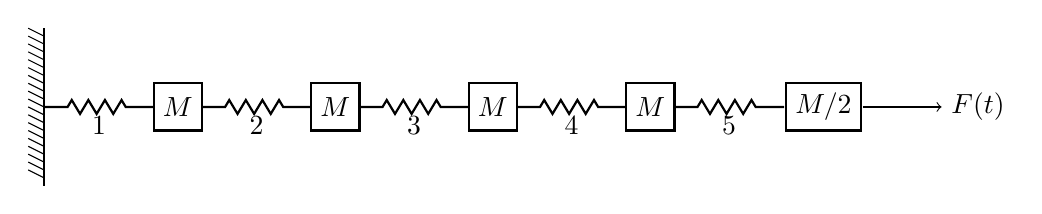
\begin{tikzpicture}

        % Wall
        \draw (-0.2, -1) -- (-0.2,  1);
        \foreach \y in {-.9, -.8, ..., .9}
        \draw (-0.2, \y) -- ++(-0.2, +0.1);

        % Bar
        \foreach \x in {0, 1, ..., 4}
            {
                \draw[spring] (2*\x-0.2, 0) -- ++(2-0.6, 0);
                \node[below] at (2*\x+0.5, 0) {$\the\numexpr\x+1\relax$};
            }

        \foreach \x in {0, 1, ..., 3}
        \node [mass] at (2*\x+1.5, 0) {$M$};

        \node [mass] at (2*4+1.5+0.2, 0) {$M/2$};

        % Force
        \draw[->] (2*4+1.5+0.2+0.5, 0) -- ++(1, 0) node[right]{$F(t)$};

    \end{tikzpicture}
    \caption{System of masses and springs equivalent to the 5 element FEM discretization of the rod with diagonalized mass matrix}
    \label{fig:masses_and_springs}

\end{figure}

In particular, given that we have diagonalized the mass matrix in our FEM formulation, we basically have supposed to move the mass of each FEM element to its extremities.

Notice however the subtle difference between the two systems:

\begin{itemize}
    \item FEM formulation: we are working in a discretized domain, were we are forced to use very small-time steps to capture the dynamics of the system.
    \item Mass-spring system: we are working in a continuous domain (differentiable), where the solution of the equation of motion is a continuous function of time.
\end{itemize}

